\documentclass[11pt]{article}
% \pagestyle{empty}

\setlength{\oddsidemargin}{-0.25 in}
\setlength{\evensidemargin}{-0.25 in}
\setlength{\topmargin}{-0.9 in}
\setlength{\textwidth}{7.0 in}
\setlength{\textheight}{9.0 in}
\setlength{\headsep}{0.75 in}
\setlength{\parindent}{0.3 in}
\setlength{\parskip}{0.1 in}
\usepackage{epsf}
\usepackage{pseudocode}
\usepackage{ amssymb }
\usepackage{tikz}
\usepackage{listings}
\usetikzlibrary{arrows.meta}
\usepackage{algorithmic}
\usepackage{changepage}
\usepackage{lipsum}
\usepackage{enumitem}
\usepackage{indentfirst}
\usepackage{amsmath}
\usepackage{graphicx}
\graphicspath{ {desktop/} }


% \usepackage{times}
% \usepackage{mathptm}

\def\O{\mathop{\smash{O}}\nolimits}
\def\o{\mathop{\smash{o}}\nolimits}
\newcommand{\e}{{\rm e}}
\newcommand{\R}{{\bf R}}
\newcommand{\Z}{{\bf Z}}
\newcommand{\findent}{\leavevmode{\parindent=2em\indent}}
\newcommand\solution{%
  \textbf{Solution.}\\%
}
\begin{document}

CS 124 Problem Set 6 \\
\indent HARVARD ID: 10939860

\begin{enumerate}

\item

\solution \\
To find the expected number of moves, we will find a recurrence. Letting $E_i$ be the expected number of moves to reach $n$ starting from position $i$, we can write out the first few values of the recurrences to find a pattern. We simply use the problem's instructions for the random walk:
\begin{equation*}
  E_0 = \frac{1}{2}E_0 + \frac{1}{2}E_1 + 1
\end{equation*}
\begin{equation*}
  E_1 = \frac{1}{2}E_0 + \frac{1}{2}E_2 + 1
\end{equation*}
\begin{equation*}
  E_2 = \frac{1}{2}E_1 + \frac{1}{2}E_3 + 1
\end{equation*}
\begin{equation*}
  E_3 = \frac{1}{2}E_2 + \frac{1}{2}E_4 + 1
\end{equation*}
which we can generalize to 
\begin{equation*}
  E_i = \frac{1}{2}(E_{i-1} + E_{i+1}) + 1
\end{equation*}

We can solve for $E_1$ in terms of $E_0$ from the first equation and then plug in to the second equation to solve for $E_2$:
\begin{equation*}
  \frac{1}{2}E_0 - 1 = \frac{1}{2}E_1
\end{equation*}
\begin{equation*}
  E_1 = 2(\frac{1}{2}E_0 - 1) = E_0 - 2
\end{equation*}
\begin{equation*}
  E_0 - 2 = \frac{1}{2}E_0 + \frac{1}{2}E_2 + 1
\end{equation*}
\begin{equation*}
  \frac{1}{2}E_0 - 3 = \frac{1}{2}E_2
\end{equation*}
\begin{equation*}
  E_2 = E_0 - 6
\end{equation*}

Using the same logic for the following equations by plugging in each equation to the next, we get that 
\begin{equation*}
  E_3 = E_0 - 12
\end{equation*}
\begin{equation*}
  E_4 = E_0 - 20
\end{equation*}

By pattern recognition, we notice that 
\begin{equation*}
  E_i = E_0 - (i^2 + i)
\end{equation*}
Since we know that $E_n = 0$, we plug in $n$ to this recurrence:
\begin{equation*}
  0 = E_0 - (n^2 + n)
\end{equation*}
\begin{equation*}
  E_0 = n^2 + n
\end{equation*}

So,
\begin{equation*}
  E_i = (n^2 + n) - (i^2 + i) = (n^2 + n) - i(i+1)
\end{equation*}

We will use the second form of the solution to prove that our solution to the recurrence is correct. Using this as our base case, we will prove correctness by induction, showing that $E_{i+1}$ is equal to the next iteration of $(n^2 + n) - i(i+1)$:
\begin{equation*}
  E_{i+1} = (n^2 + n) - (i+1)^2 - (i+1)
\end{equation*}
\begin{equation*}
  = n^2 +n - i^2 - 3i - 2
\end{equation*}
\begin{equation*}
  = n^2 + n - (i+2)(i+1)
\end{equation*}
Our solution shows that $E_{i+1} = n^2 + n - (i+2)(i+1) = n^2 + n - ((i+1)+2)(i+1)$, and thus the recurrence is correct for all $n, i \geq 0$. 


\item

\solution \\
To find the minimum flow between $s$ and $t$, we will run the Ford-Fulkerson algorithm, drawing the residual graph at each step. The max flow in step 1 with path $s -> c -> a -> e -> t$ is 1: 
\begin{center}
\begin{tikzpicture}[scale=0.2]
\tikzstyle{every node}+=[inner sep=0pt]
\draw [black] (12.2,-27.8) circle (3);
\draw (12.2,-27.8) node {$s$};
\draw [black] (27,-12.1) circle (3);
\draw (27,-12.1) node {$a$};
\draw [black] (47,-12.1) circle (3);
\draw (47,-12.1) node {$b$};
\draw [black] (47,-27.2) circle (3);
\draw (47,-27.2) node {$e$};
\draw [black] (64.4,-27.2) circle (3);
\draw (64.4,-27.2) node {$t$};
\draw [black] (27,-42.6) circle (3);
\draw (27,-42.6) node {$c$};
\draw [black] (47,-42.6) circle (3);
\draw (47,-42.6) node {$d$};
\draw [black] (14.26,-25.62) -- (24.94,-14.28);
\fill [black] (24.94,-14.28) -- (24.03,-14.52) -- (24.76,-15.21);
\draw (20.13,-21.42) node [right] {$4$};
\draw [black] (30,-12.1) -- (44,-12.1);
\fill [black] (44,-12.1) -- (43.2,-11.6) -- (43.2,-12.6);
\draw (37,-12.6) node [below] {$3$};
\draw [black] (49.27,-14.07) -- (62.13,-25.23);
\fill [black] (62.13,-25.23) -- (61.86,-24.33) -- (61.2,-25.09);
\draw (54.69,-20.14) node [below] {$4$};
\draw [black] (24.468,-40.993) arc (-124.47954:-145.52046:41.285);
\fill [black] (24.47,-40.99) -- (24.09,-40.13) -- (23.52,-40.95);
\draw (17.62,-36.63) node [below] {$4$};
\draw [black] (14.732,-29.407) arc (55.52046:34.47954:41.285);
\fill [black] (14.73,-29.41) -- (15.11,-30.27) -- (15.68,-29.45);
\draw (21.58,-33.77) node [above] {$1$};
\draw [black] (26.611,-39.625) arc (-173.3577:-186.6423:106.124);
\fill [black] (26.61,-39.63) -- (27.02,-38.77) -- (26.02,-38.89);
\draw (25.4,-27.35) node [left] {$1$};
\draw [black] (27.528,-15.053) arc (9.0392:-9.0392:78.27);
\fill [black] (27.53,-15.05) -- (27.16,-15.92) -- (28.15,-15.76);
\draw (29,-27.35) node [right] {$0$};
\draw [black] (30,-42.6) -- (44,-42.6);
\fill [black] (44,-42.6) -- (43.2,-42.1) -- (43.2,-43.1);
\draw (37,-43.1) node [below] {$3$};
\draw [black] (29.38,-40.77) -- (44.62,-29.03);
\fill [black] (44.62,-29.03) -- (43.68,-29.12) -- (44.29,-29.91);
\draw (38.01,-35.4) node [below] {$1$};
\draw [black] (28.65,-14.61) -- (45.35,-40.09);
\fill [black] (45.35,-40.09) -- (45.33,-39.15) -- (44.5,-39.7);
\draw (36.38,-28.67) node [left] {$2$};
\draw [black] (44.4,-25.704) arc (-120.88891:-133.2167:88.974);
\fill [black] (44.4,-25.7) -- (43.97,-24.86) -- (43.46,-25.72);
\draw (35.46,-20.85) node [below] {$0$};
\draw [black] (29.671,-13.466) arc (61.56355:44.33084:63.915);
\fill [black] (29.67,-13.47) -- (30.14,-14.29) -- (30.61,-13.41);
\draw (38.75,-18.16) node [above] {$1$};
\draw [black] (49.943,-26.62) arc (98.85761:81.14239:37.391);
\fill [black] (61.46,-26.62) -- (60.74,-26) -- (60.59,-26.99);
\draw (55.7,-25.67) node [above] {$1$};
\draw [black] (61.466,-27.821) arc (-80.5041:-99.4959:34.95);
\fill [black] (49.93,-27.82) -- (50.64,-28.45) -- (50.81,-27.46);
\draw (55.7,-28.8) node [below] {$1$};
\draw [black] (49.25,-40.61) -- (62.15,-29.19);
\fill [black] (62.15,-29.19) -- (61.22,-29.34) -- (61.89,-30.09);
\draw (56.71,-35.39) node [below] {$3$};
\end{tikzpicture}
\end{center}

The max flow at step 2 with path $s -> a -> b -> t$ is 3: 

\begin{center}
\begin{tikzpicture}[scale=0.2]
\tikzstyle{every node}+=[inner sep=0pt]
\draw [black] (12.2,-27.8) circle (3);
\draw (12.2,-27.8) node {$s$};
\draw [black] (27,-12.1) circle (3);
\draw (27,-12.1) node {$a$};
\draw [black] (47,-12.1) circle (3);
\draw (47,-12.1) node {$b$};
\draw [black] (47,-27.2) circle (3);
\draw (47,-27.2) node {$e$};
\draw [black] (64.4,-27.2) circle (3);
\draw (64.4,-27.2) node {$t$};
\draw [black] (27,-42.6) circle (3);
\draw (27,-42.6) node {$c$};
\draw [black] (47,-42.6) circle (3);
\draw (47,-42.6) node {$d$};
\draw [black] (25.288,-14.563) arc (-36.16983:-50.44976:62.926);
\fill [black] (25.29,-14.56) -- (24.41,-14.91) -- (25.22,-15.5);
\draw (20.81,-22.06) node [right] {$1$};
\draw [black] (44.021,-12.457) arc (-84.37235:-95.62765:71.602);
\fill [black] (44.02,-12.46) -- (43.18,-12.04) -- (43.27,-13.03);
\draw (37,-13.3) node [below] {$0$};
\draw [black] (61.904,-25.536) arc (-124.78051:-137.12343:79.471);
\fill [black] (61.9,-25.54) -- (61.53,-24.67) -- (60.96,-25.49);
\draw (54.14,-20.77) node [below] {$1$};
\draw [black] (24.468,-40.993) arc (-124.47954:-145.52046:41.285);
\fill [black] (24.47,-40.99) -- (24.09,-40.13) -- (23.52,-40.95);
\draw (17.62,-36.63) node [below] {$4$};
\draw [black] (14.732,-29.407) arc (55.52046:34.47954:41.285);
\fill [black] (14.73,-29.41) -- (15.11,-30.27) -- (15.68,-29.45);
\draw (21.58,-33.77) node [above] {$1$};
\draw [black] (26.611,-39.625) arc (-173.3577:-186.6423:106.124);
\fill [black] (26.61,-39.63) -- (27.02,-38.77) -- (26.02,-38.89);
\draw (25.4,-27.35) node [left] {$1$};
\draw [black] (27.528,-15.053) arc (9.0392:-9.0392:78.27);
\fill [black] (27.53,-15.05) -- (27.16,-15.92) -- (28.15,-15.76);
\draw (29,-27.35) node [right] {$0$};
\draw [black] (30,-42.6) -- (44,-42.6);
\fill [black] (44,-42.6) -- (43.2,-42.1) -- (43.2,-43.1);
\draw (37,-43.1) node [below] {$3$};
\draw [black] (29.38,-40.77) -- (44.62,-29.03);
\fill [black] (44.62,-29.03) -- (43.68,-29.12) -- (44.29,-29.91);
\draw (38.01,-35.4) node [below] {$1$};
\draw [black] (28.65,-14.61) -- (45.35,-40.09);
\fill [black] (45.35,-40.09) -- (45.33,-39.15) -- (44.5,-39.7);
\draw (36.38,-28.67) node [left] {$2$};
\draw [black] (44.4,-25.704) arc (-120.88891:-133.2167:88.974);
\fill [black] (44.4,-25.7) -- (43.97,-24.86) -- (43.46,-25.72);
\draw (35.46,-20.85) node [below] {$0$};
\draw [black] (29.671,-13.466) arc (61.56355:44.33084:63.915);
\fill [black] (29.67,-13.47) -- (30.14,-14.29) -- (30.61,-13.41);
\draw (38.75,-18.16) node [above] {$1$};
\draw [black] (49.943,-26.62) arc (98.85761:81.14239:37.391);
\fill [black] (61.46,-26.62) -- (60.74,-26) -- (60.59,-26.99);
\draw (55.7,-25.67) node [above] {$1$};
\draw [black] (61.466,-27.821) arc (-80.5041:-99.4959:34.95);
\fill [black] (49.93,-27.82) -- (50.64,-28.45) -- (50.81,-27.46);
\draw (55.7,-28.8) node [below] {$1$};
\draw [black] (49.25,-40.61) -- (62.15,-29.19);
\fill [black] (62.15,-29.19) -- (61.22,-29.34) -- (61.89,-30.09);
\draw (56.71,-35.39) node [below] {$3$};
\draw [black] (13.622,-25.159) arc (149.31927:124.06114:36.093);
\fill [black] (13.62,-25.16) -- (14.46,-24.73) -- (13.6,-24.22);
\draw (17.87,-17.35) node [left] {$3$};
\draw [black] (29.947,-11.544) arc (98.82177:81.17823:45.987);
\fill [black] (29.95,-11.54) -- (30.81,-11.91) -- (30.66,-10.93);
\draw (37,-10.5) node [above] {$3$};
\draw [black] (49.674,-13.458) arc (61.00946:37.08659:41.54);
\fill [black] (49.67,-13.46) -- (50.13,-14.28) -- (50.62,-13.41);
\draw (57.78,-17.93) node [above] {$3$};
\end{tikzpicture}
\end{center}

The max flow in step 3 with path $s -> c -> d -> t$ is 3: 

\begin{center}
\begin{tikzpicture}[scale=0.2]
\tikzstyle{every node}+=[inner sep=0pt]
\draw [black] (12.2,-27.8) circle (3);
\draw (12.2,-27.8) node {$s$};
\draw [black] (27,-12.1) circle (3);
\draw (27,-12.1) node {$a$};
\draw [black] (47,-12.1) circle (3);
\draw (47,-12.1) node {$b$};
\draw [black] (47,-27.2) circle (3);
\draw (47,-27.2) node {$e$};
\draw [black] (64.4,-27.2) circle (3);
\draw (64.4,-27.2) node {$t$};
\draw [black] (27,-42.6) circle (3);
\draw (27,-42.6) node {$c$};
\draw [black] (47,-42.6) circle (3);
\draw (47,-42.6) node {$d$};
\draw [black] (25.288,-14.563) arc (-36.16983:-50.44976:62.926);
\fill [black] (25.29,-14.56) -- (24.41,-14.91) -- (25.22,-15.5);
\draw (20.81,-22.06) node [right] {$1$};
\draw [black] (44.021,-12.457) arc (-84.37235:-95.62765:71.602);
\fill [black] (44.02,-12.46) -- (43.18,-12.04) -- (43.27,-13.03);
\draw (37,-13.3) node [below] {$0$};
\draw [black] (61.904,-25.536) arc (-124.78051:-137.12343:79.471);
\fill [black] (61.9,-25.54) -- (61.53,-24.67) -- (60.96,-25.49);
\draw (54.14,-20.77) node [below] {$1$};
\draw [black] (24.468,-40.993) arc (-124.47954:-145.52046:41.285);
\fill [black] (24.47,-40.99) -- (24.09,-40.13) -- (23.52,-40.95);
\draw (17.62,-36.63) node [below] {$1$};
\draw [black] (14.732,-29.407) arc (55.52046:34.47954:41.285);
\fill [black] (14.73,-29.41) -- (15.11,-30.27) -- (15.68,-29.45);
\draw (21.58,-33.77) node [above] {$4$};
\draw [black] (26.611,-39.625) arc (-173.3577:-186.6423:106.124);
\fill [black] (26.61,-39.63) -- (27.02,-38.77) -- (26.02,-38.89);
\draw (25.4,-27.35) node [left] {$1$};
\draw [black] (27.528,-15.053) arc (9.0392:-9.0392:78.27);
\fill [black] (27.53,-15.05) -- (27.16,-15.92) -- (28.15,-15.76);
\draw (29,-27.35) node [right] {$0$};
\draw [black] (29.956,-42.093) arc (98.02065:81.97935:50.48);
\fill [black] (44.04,-42.09) -- (43.32,-41.49) -- (43.18,-42.48);
\draw (37,-41.1) node [above] {$0$};
\draw [black] (29.38,-40.77) -- (44.62,-29.03);
\fill [black] (44.62,-29.03) -- (43.68,-29.12) -- (44.29,-29.91);
\draw (38.01,-35.4) node [below] {$1$};
\draw [black] (28.65,-14.61) -- (45.35,-40.09);
\fill [black] (45.35,-40.09) -- (45.33,-39.15) -- (44.5,-39.7);
\draw (36.38,-28.67) node [left] {$2$};
\draw [black] (44.4,-25.704) arc (-120.88891:-133.2167:88.974);
\fill [black] (44.4,-25.7) -- (43.97,-24.86) -- (43.46,-25.72);
\draw (35.46,-20.85) node [below] {$0$};
\draw [black] (29.671,-13.466) arc (61.56355:44.33084:63.915);
\fill [black] (29.67,-13.47) -- (30.14,-14.29) -- (30.61,-13.41);
\draw (38.75,-18.16) node [above] {$1$};
\draw [black] (49.943,-26.62) arc (98.85761:81.14239:37.391);
\fill [black] (61.46,-26.62) -- (60.74,-26) -- (60.59,-26.99);
\draw (55.7,-25.67) node [above] {$1$};
\draw [black] (61.466,-27.821) arc (-80.5041:-99.4959:34.95);
\fill [black] (49.93,-27.82) -- (50.64,-28.45) -- (50.81,-27.46);
\draw (55.7,-28.8) node [below] {$1$};
\draw [black] (48.825,-40.22) arc (140.90009:122.12126:53.166);
\fill [black] (61.82,-28.72) -- (60.87,-28.72) -- (61.4,-29.57);
\draw (53.84,-33.45) node [above] {$0$};
\draw [black] (13.622,-25.159) arc (149.31927:124.06114:36.093);
\fill [black] (13.62,-25.16) -- (14.46,-24.73) -- (13.6,-24.22);
\draw (17.87,-17.35) node [left] {$3$};
\draw [black] (29.947,-11.544) arc (98.82177:81.17823:45.987);
\fill [black] (29.95,-11.54) -- (30.81,-11.91) -- (30.66,-10.93);
\draw (37,-10.5) node [above] {$3$};
\draw [black] (49.674,-13.458) arc (61.00946:37.08659:41.54);
\fill [black] (49.67,-13.46) -- (50.13,-14.28) -- (50.62,-13.41);
\draw (57.78,-17.93) node [above] {$3$};
\draw [black] (44.085,-43.304) arc (-78.77671:-101.22329:36.401);
\fill [black] (29.92,-43.3) -- (30.6,-43.95) -- (30.8,-42.97);
\draw (37,-44.5) node [below] {$3$};
\draw [black] (62.701,-29.672) arc (-36.55068:-60.42797:42.093);
\fill [black] (49.66,-41.21) -- (50.6,-41.25) -- (50.11,-40.38);
\draw (57.8,-36.61) node [below] {$3$};
\end{tikzpicture}
\end{center}

And finally, the max flow at step 4 with step $s -> a -> c -> e -> t$, the final step in the algorithm, is 1:
\begin{center}
\begin{tikzpicture}[scale=0.2]
\tikzstyle{every node}+=[inner sep=0pt]
\draw [black] (12.2,-27.8) circle (3);
\draw (12.2,-27.8) node {$s$};
\draw [black] (27,-12.1) circle (3);
\draw (27,-12.1) node {$a$};
\draw [black] (47,-12.1) circle (3);
\draw (47,-12.1) node {$b$};
\draw [black] (47,-27.2) circle (3);
\draw (47,-27.2) node {$e$};
\draw [black] (64.4,-27.2) circle (3);
\draw (64.4,-27.2) node {$t$};
\draw [black] (27,-42.6) circle (3);
\draw (27,-42.6) node {$c$};
\draw [black] (47,-42.6) circle (3);
\draw (47,-42.6) node {$d$};
\draw [black] (25.288,-14.563) arc (-36.16983:-50.44976:62.926);
\fill [black] (25.29,-14.56) -- (24.41,-14.91) -- (25.22,-15.5);
\draw (20.81,-22.06) node [right] {$0$};
\draw [black] (44.021,-12.457) arc (-84.37235:-95.62765:71.602);
\fill [black] (44.02,-12.46) -- (43.18,-12.04) -- (43.27,-13.03);
\draw (37,-13.3) node [below] {$0$};
\draw [black] (61.904,-25.536) arc (-124.78051:-137.12343:79.471);
\fill [black] (61.9,-25.54) -- (61.53,-24.67) -- (60.96,-25.49);
\draw (54.14,-20.77) node [below] {$1$};
\draw [black] (24.468,-40.993) arc (-124.47954:-145.52046:41.285);
\fill [black] (24.47,-40.99) -- (24.09,-40.13) -- (23.52,-40.95);
\draw (17.62,-36.63) node [below] {$1$};
\draw [black] (14.732,-29.407) arc (55.52046:34.47954:41.285);
\fill [black] (14.73,-29.41) -- (15.11,-30.27) -- (15.68,-29.45);
\draw (21.58,-33.77) node [above] {$4$};
\draw [black] (26.611,-39.625) arc (-173.3577:-186.6423:106.124);
\fill [black] (26.61,-39.63) -- (27.02,-38.77) -- (26.02,-38.89);
\draw (25.4,-27.35) node [left] {$0$};
\draw [black] (27.563,-15.046) arc (9.65189:-9.65189:73.383);
\fill [black] (27.56,-15.05) -- (27.2,-15.92) -- (28.19,-15.75);
\draw (29.1,-27.35) node [right] {$1$};
\draw [black] (29.956,-42.093) arc (98.02065:81.97935:50.48);
\fill [black] (44.04,-42.09) -- (43.32,-41.49) -- (43.18,-42.48);
\draw (37,-41.1) node [above] {$0$};
\draw [black] (44.883,-29.326) arc (-45.89211:-58.91535:85.067);
\fill [black] (44.88,-29.33) -- (43.96,-29.52) -- (44.66,-30.24);
\draw (38.58,-36.14) node [below] {$0$};
\draw [black] (28.65,-14.61) -- (45.35,-40.09);
\fill [black] (45.35,-40.09) -- (45.33,-39.15) -- (44.5,-39.7);
\draw (36.38,-28.67) node [left] {$2$};
\draw [black] (44.4,-25.704) arc (-120.88891:-133.2167:88.974);
\fill [black] (44.4,-25.7) -- (43.97,-24.86) -- (43.46,-25.72);
\draw (35.46,-20.85) node [below] {$0$};
\draw [black] (29.671,-13.466) arc (61.56355:44.33084:63.915);
\fill [black] (29.67,-13.47) -- (30.14,-14.29) -- (30.61,-13.41);
\draw (38.75,-18.16) node [above] {$1$};
\draw [black] (49.943,-26.62) arc (98.85761:81.14239:37.391);
\fill [black] (61.46,-26.62) -- (60.74,-26) -- (60.59,-26.99);
\draw (55.7,-25.67) node [above] {$0$};
\draw [black] (61.466,-27.821) arc (-80.5041:-99.4959:34.95);
\fill [black] (49.93,-27.82) -- (50.64,-28.45) -- (50.81,-27.46);
\draw (55.7,-28.8) node [below] {$2$};
\draw [black] (48.825,-40.22) arc (140.90009:122.12126:53.166);
\fill [black] (61.82,-28.72) -- (60.87,-28.72) -- (61.4,-29.57);
\draw (53.84,-33.45) node [above] {$0$};
\draw [black] (13.622,-25.159) arc (149.31927:124.06114:36.093);
\fill [black] (13.62,-25.16) -- (14.46,-24.73) -- (13.6,-24.22);
\draw (17.87,-17.35) node [left] {$4$};
\draw [black] (29.947,-11.544) arc (98.82177:81.17823:45.987);
\fill [black] (29.95,-11.54) -- (30.81,-11.91) -- (30.66,-10.93);
\draw (37,-10.5) node [above] {$3$};
\draw [black] (49.674,-13.458) arc (61.00946:37.08659:41.54);
\fill [black] (49.67,-13.46) -- (50.13,-14.28) -- (50.62,-13.41);
\draw (57.78,-17.93) node [above] {$3$};
\draw [black] (44.085,-43.304) arc (-78.77671:-101.22329:36.401);
\fill [black] (29.92,-43.3) -- (30.6,-43.95) -- (30.8,-42.97);
\draw (37,-44.5) node [below] {$3$};
\draw [black] (62.701,-29.672) arc (-36.55068:-60.42797:42.093);
\fill [black] (49.66,-41.21) -- (50.6,-41.25) -- (50.11,-40.38);
\draw (57.8,-36.61) node [below] {$3$};
\draw [black] (29.095,-40.453) arc (134.60784:120.5847:79.062);
\fill [black] (29.1,-40.45) -- (30.02,-40.25) -- (29.31,-39.54);
\draw (35.38,-33.6) node [above] {$1$};
\end{tikzpicture}
\end{center}

Now, our algorithm is finished because a path can no longer be found from $s$ to $t$ with sufficient flow. Thus, adding the max flows in each of the residual steps, we find that the maximum flow from $s$ to $t$ is 8. \\
\\
To find the minimum cut, we find the vertices that are reachable from start node $s$, so we have our cut to be $S = \{s, c, a, d\}$, with $V-S = \{b, e, t\}$. We can confirm that this is the minimum cut, since the capacities going into the cut is equal to that of the maximum flow, which makes sense, since all flow must cross the cut at some point. Adding the flow from the given graph of edges that cross into the cut from $S$ into $V-S$, we have $c_{ab} + c_{ae}+c_{ce}+c_{dt} = 3 + 3 + 1 + 1 = 8$, which we have found to be the maximum flow, so the given cut is indeed the minimum cut. 


\item 

\solution \\
We can set this up as a flow problem, with a similar setup to the hospital and patient problem discussed in section. Consider the graph shown below. There are $2n + 2$ nodes in total, with $s$, a source node, $t$, a sink node, $r_1, ..., r_n$ representing the $i^{th}$ row, and $c_1, ..., c_n$ representing the $j^{th}$ column. This is a rudimentary example to show a representation of a plot with 3 rows and 3 columns:

\begin{center}
\begin{tikzpicture}[scale=0.2]
\tikzstyle{every node}+=[inner sep=0pt]
\draw [black] (11.4,-28.1) circle (3);
\draw (11.4,-28.1) node {$s$};
\draw [black] (25.6,-15.4) circle (3);
\draw (25.6,-15.4) node {$r_1$};
\draw [black] (25.6,-28.1) circle (3);
\draw (25.6,-28.1) node {$r_2$};
\draw [black] (25.6,-41) circle (3);
\draw (25.6,-41) node {$r_3$};
\draw [black] (48.4,-41) circle (3);
\draw (48.4,-41) node {$c_3$};
\draw [black] (48.4,-28.1) circle (3);
\draw (48.4,-28.1) node {$c_2$};
\draw [black] (48.4,-15.4) circle (3);
\draw (48.4,-15.4) node {$c_1$};
\draw [black] (65.6,-28.1) circle (3);
\draw (65.6,-28.1) node {$t$};
\draw [black] (13.64,-26.1) -- (23.36,-17.4);
\fill [black] (23.36,-17.4) -- (22.43,-17.56) -- (23.1,-18.31);
\draw (19.51,-22.24) node [below] {$x$};
\draw [black] (14.4,-28.1) -- (22.6,-28.1);
\fill [black] (22.6,-28.1) -- (21.8,-27.6) -- (21.8,-28.6);
\draw (18.5,-28.6) node [below] {$x$};
\draw [black] (13.62,-30.12) -- (23.38,-38.98);
\fill [black] (23.38,-38.98) -- (23.12,-38.07) -- (22.45,-38.81);
\draw (17.49,-35.04) node [below] {$x$};
\draw [black] (28.6,-15.4) -- (45.4,-15.4);
\fill [black] (45.4,-15.4) -- (44.6,-14.9) -- (44.6,-15.9);
\draw (37,-15.9) node [below] {$1$};
\draw [black] (28.22,-16.86) -- (45.78,-26.64);
\fill [black] (45.78,-26.64) -- (45.32,-25.81) -- (44.84,-26.69);
\draw (36,-22.25) node [below] {$1$};
\draw [black] (27.6,-17.64) -- (46.4,-38.76);
\fill [black] (46.4,-38.76) -- (46.25,-37.83) -- (45.5,-38.49);
\draw (36.46,-29.65) node [left] {$1$};
\draw [black] (28.6,-28.1) -- (45.4,-28.1);
\fill [black] (45.4,-28.1) -- (44.6,-27.6) -- (44.6,-28.6);
\draw [black] (27.6,-38.76) -- (46.4,-17.64);
\fill [black] (46.4,-17.64) -- (45.5,-17.91) -- (46.25,-18.57);
\draw (37.54,-29.65) node [right] {$1$};
\draw [black] (28.6,-41) -- (45.4,-41);
\fill [black] (45.4,-41) -- (44.6,-40.5) -- (44.6,-41.5);
\draw (37,-41.5) node [below] {$1$};
\draw [black] (50.81,-17.18) -- (63.19,-26.32);
\fill [black] (63.19,-26.32) -- (62.84,-25.44) -- (62.25,-26.25);
\draw (56,-22.25) node [below] {$x$};
\draw [black] (51.4,-28.1) -- (62.6,-28.1);
\fill [black] (62.6,-28.1) -- (61.8,-27.6) -- (61.8,-28.6);
\draw (57,-28.6) node [below] {$x$};
\draw [black] (50.8,-39.2) -- (63.2,-29.9);
\fill [black] (63.2,-29.9) -- (62.26,-29.98) -- (62.86,-30.78);
\draw (58,-35.05) node [below] {$x$};
\end{tikzpicture}
\end{center}

In this representation, the edge from $r_i$ to $c_j$ gives the subplot of the $r_i c_j$ location on the plot of land. The 1 value attached to the edge can be thought of a boolean value. If there exists an edge with capacity 1 in subplot $r_i c_j$ (because each subplot can only hold one tree), then that subplot has soil and can support plant growth. If subplot $r_i c_j$ has rocky ground and cannot support the growth of a tree, then there is an edge between $r_i$ and $c_j$ with capacity 0, though for simplicity those edges have been left out of the above graph, since they are irrelevant. \\
\\
The value of $x$ in the graph will ultimately be $p$, which we are trying to maximize. With this setup, we treat $x$ as a counter that will give us the maximum value for $p$ that maintains the restrictions given by the problem. To do this, set $x$ as 1, run the Ford-Fulkerson algorithm to completion, and check if all edges going into the sink node $t$ are used to their full capacity (left with 0). If this condition is met, run Ford-Fulkerson on the graph again with $x = 2$. Continue this, incrementing $x$ by 1 each time until the algorithm does not use up all capacity of the edges with $x$ capacity originally. When this happens, set $p$ to be the final $p$ where Ford-Fulkerson gave the result of all capacity being used. The final precise plot will have trees in all subplots with an edge that has capacity 1. \\
\\
This algorithm works because it makes sure that every row and column has the same number of trees, which is $p$, because of the orientation of the graph. $p$ will always stay the same for all rows and columns since $x$ is associated with many edges and we update them collectively. We also know that $p$ will be maximized because we take the final value for $x$ that is "successful"; that is, the largest value that makes sure that the number of trees and columns is still the same before that condition can no longer be met. \\
\\
The runtime for this algorithm is the runtime of Ford-Fulkerson, which is $O(f^*E)$. Here, our max flow ($f^*$) is $n^2$, due to the possible number of edges from $r_1, ..., r_n$ and $c_1, ..., c_n$. The number of edges (E) is $n^2 + n$, for the $n^2$ possible edges just stated added to the $2n$ edges between the source to the rest of the graph and the graph to the sink. Thus, the runtime for this algorithm is $O(n^2(n^2 + 2n)) = O(n^4)$. 

\item 

\solution \begin{itemize}
\item
We can simply formulate this adopted network flow problem into a linear program. Letting $f_{uv}$ be the amount of flow between two nodes on the edge $(u,v)$, and $c_{uv}$ be the capacity of the edge $(u,v)$, we set up the following LP goal and constraints. \\
\\
\textbf{Goal}: 
\begin{equation*}
  max \sum_{i} f_{si}
\end{equation*}
\textbf{Constraints}:
\begin{equation*}
  f_{uv} \leq c_{uv}
\end{equation*}
\begin{equation*}
  f_{uv} \geq 0
\end{equation*}
And for every vertex $w$ besides $w = s$ and $w = t$,
\begin{equation*}
  \frac{1}{2} \sum_{(u,w)} f_{uw} - \sum_{(w,v)} f_{wv} = 0
\end{equation*}

These constraints are logical: for capacity, we say that the flow of an edge must be less than or equal to its capacity; for nonnegativity, we say that the flow of an edge must be at least 0; and for conservation, which is what makes this different than a typical network flow problem, we say that half of the flow into all edges must equal the flow that comes out. 
\\
\item
For this question, we take a similar approach. We let $f_{uv}$ be the amount of flow between two nodes on the edge $(u,v)$, and let $c_{uv}$ be the capacity of the edge $(u,v)$ (using $cap$ instead of $c$ since we use $c$ for the cost in this problem), and $c_e$ is the fixed cost for each unit of flow through the edge $e$. We will use two LP problems to solve. First, we maximize the flow going through the graph, which is illustrated below: \\
\\
\textbf{Goal}: 
\begin{equation*}
  max \sum_{i} f_{si}
\end{equation*}
\textbf{Constraints}:
\begin{equation*}
  f_{uv} \leq cap_{uv}
\end{equation*}
\begin{equation*}
  f_{uv} \geq 0
\end{equation*}
And for every vertex $w$ besides $w = s$ and $w = t$,
\begin{equation*}
  \sum_{(u,w)} f_{uw} - \sum_{(w,v)} f_{wv} = 0
\end{equation*}

This will give us the maximum flow. From here, set the answer to this LP problem, $max \sum_{i} f_{si}$, equal to some constant $x$ for future reference. Next, we will use a second LP program to minimize the cost of the maximum flow. Consider the following linear program: \\
\\
\textbf{Goal}: 
\begin{equation*}
  min \sum_{(u,v)} c_{uv} * f_{uv}
\end{equation*}
\textbf{Constraints}:
\begin{equation*}
  f_{uv} \leq cap_{uv}
\end{equation*}
\begin{equation*}
  f_{uv} \geq 0
\end{equation*}
And for every vertex $w$ besides $w = s$ and $w = t$,
\begin{equation*}
  \sum_{(u,w)} f_{uw} - \sum_{(w,v)} f_{wv} = 0
\end{equation*}
\begin{equation*}
  \sum_{i} f_{si} = x
\end{equation*}

The last constraint guarantees correctness, because it ensures that the only paths that are taken are paths that have flow equal to the maximum flow, and we then minimize the cost per unit of those paths. 

\end{itemize}

\item 

\solution \\
To create a linear time algorithm to compute the new maximum flow after adding 1 to a given edge $e$, we will assume that we are given the final residual after running an algorithm such as Ford-Fulkerson, and we will work with that graph. \\
\\
After adding 1 to a certain edge in the final residual graph, there are two options. This will either give a new path possible from $s$ to $t$ (where $s$ is the source and $t$ is the sink), which will happen if the edge in the residual graph was initially 0. In this case, we add one to the final max flow that we are given. In the other case, 1 is added to the capacity of an edge that can't be reached anyway in the residual graph. In this case, our given max flow does not change, since it won't be affected by this edge. \\
\\
To determine which case the given edge falls under, run a depth-first search from $s$ to $t$ in the residual graph after adding 1 to the capacity of the given edge. Since DFS can find if a path between two nodes exists, if a path from $s$ to $t$ does indeed exist, then add 1 to the max flow, and if no path exists, then return the original max flow. This algorithm works correctly because it checks if the edge that has 1 added to it affects the overall max flow or not in the original graph with DFS, determining whether or not we need to increase the max flow by 1. \\
\\
In the case where a given edge $e$ is decreased by 1, we again work with the final residual graph, and we again have two cases. In the first case, after subtracting from an edge in the residual graph, it stays greater or equal to 0, which occurs when that edge in the residual graph was initially positive. In this case, everything done up to this point was valid (that even after subtracting that edge still has the capacity to handle the amount of flow necessary). In this case, the max flow does not change. In the other case, an edge becomes negative after subtracting 1 from it, meaning that in the residual graph it was initially at a capacity of 0. In this case, something we did to find the max flow was not valid, because the algorithm must have run through an edge with 0 capacity. In this case, we must subtract one from the total max flow given. \\
\\
To determine which case the given edge falls under, we will again DFS, but this time running it backwards (from the sink to the source). If there is a valid path from $t$ to $s$, then we know that the given edge forwards must be negative, because a negative flow backwards will give a positive flow. So, if this backwards DFS finds a path, then subtract 1 from the total max flow, and if it does not find a path, then there is not a negative edge when going forwards in the graph, so return the original max flow. This algorithm works correctly, because it checks to see if a given edge is negative or not once some edge's capacity is decreased by 1, decreasing the overall max flow if an edge is negative, since the max flow would not be valid in this case.
\\
The runtime for both algorithms is simply the runtime of DFS, which is $O(|V| + |E|)$, since we are assuming that we are given the residual graph of the given graph.


\item 

\solution \\
Similar to the problem in section, let the row strategy be $(y_1, y_2, y_3, y_4)$ and the column strategy be $(x_1, x_2, x_3, x_4)$, meaning row $i$ is chosen with probability i and column $j$ is chosen with probability $x_j$. Because a positive payoff goes to the row player, we want to maximize the row strategy's expected payoff and minimize the column strategy's expected payoff. \\
\\
Consider the following linear program to maximize the row strategy, letting $a$ be the maximum payoff: \\
\\
\textbf{Goal}:
\begin{equation*}
  a = max(3y_1 + 6y_2 - 3y_3 - 7y_4, y_1 - 2y_2 - 2y_3 + 4y_4, -2y_2 + 3y_3 - 5y_4, -4y_1 - 3y_3 + 7y_4)
\end{equation*}
\textbf{Constraints:}
\begin{equation*}
  a - 3y_1 - 6y_2 + 3y_3 + 7y_4 \leq 0
\end{equation*}
\begin{equation*}
  a -  y_1 + 2y_2 + 2y_3 - 4y_4 \leq 0
\end{equation*}
\begin{equation*}
  a + 2y_2 - 3y_3 + 5y_4 \leq 0
\end{equation*}
\begin{equation*}
  a + 4y_1 + 3y_3 - 7y_4 \leq 0
\end{equation*}
\begin{equation*}
  y_1 + y_2 + y_3 + y_4 = 1
\end{equation*}

Next, we must write a linear program to minimize the column strategy, letting $b$ be the minimum payoff: \\
\\
\textbf{Goal}:
\begin{equation*}
  b = min(3x_1 + x_2 + 4x_4, 6x_1 - 2x_2 - 2x_3, -3x_1 - 2x_2 + 3x_3 - 3x_4, -7x_1 + 4x_2 - 5x_3 + 7x_4)
\end{equation*}
\textbf{Constraints:}
\begin{equation*}
  b - 3y_1 - 6y_2 + 3y_3 + 7y_4 \geq 0
\end{equation*}
\begin{equation*}
  b -  y_1 + 2y_2 + 2y_3 - 4y_4 \geq 0
\end{equation*}
\begin{equation*}
  b + 2y_2 - 3y_3 + 5y_4 \geq 0
\end{equation*}
\begin{equation*}
  b + 4y_1 + 3y_3 - 7y_4 \geq 0
\end{equation*}
\begin{equation*}
  x_1 + x_2 + x_3 + x_4 = 1
\end{equation*}

I plugged these equations into Mathematica to act as an LP solver. I got the row player's strategy as:
\begin{equation*}
  (y_1 = 8/53, y_2 = 161/583, y_3 = 221/583, y_4 = 113/583) 
\end{equation*}
and the column player's strategy as:
\begin{equation*}
  (x_1 = 81/583, x_2 = 11/53, x_ 3 = 234/583, x_4 = 147/583)
\end{equation*}

Mathematica shows that the total value or equilibrium of the game was -224/583, meaning that the game is biased to the column player, and that the row player always has a tendency to lose. Thus, since the game is fair when the equilibrium is 0, the column player should compensate the row player 224/583 units in order to make the game fair. 
\\\\\\\\\\\\\\\\\\\\\\\\\\\\\\\\

I collaborated on this problem set with Nathan Lee, Sam Bieler, and Kate Schember. 


\end{enumerate}
\end{document}
